

%% this section contains XX problems
%%----------------------------------------


%% Jacobs 5 steps to a 5
%%------------------------------
\element{AP}{
\begin{question}{Jacobs-Q20}
    Which of the following will increase the capacitance of
        a parellel plate capacitor?
    \begin{choices}
        \wrongchoice{increasing the charge stored on the plates.}
        \wrongchoice{decreasing the charge stored on the plates.}
      \correctchoice{increasing the separation between the plates.}
        \wrongchoice{decreasing the separation between the plates.}
        \wrongchoice{decreasing the area of the plates.}
    \end{choices}
\end{question}
}

\element{AP}{
\begin{question}{Jacobs-Q21}
    A \SI{10}{\volt} battery is connected to two parallel
        \SI{10}{\ohm} resistors, as shown below.
    %% NOTE: add circuit diagram
    %\begin{center}
    %    \begin{circuitikz}
    %    \end{circuitikz}
    %\end{center}
    What is the current through and voltage across each resistor?
    \begin{choices}
        \wrongchoice{\SI{1}{\ampere} and \SI{5}{\volt}}
      \correctchoice{\SI{1}{\ampere} and \SI{10}{\volt}}
        \wrongchoice{\SI{0.5}{\ampere} and \SI{5}{\volt}}
        \wrongchoice{\SI{2}{\ampere} and \SI{10}{\volt}}
        \wrongchoice{\SI{2}{\ampere} and \SI{5}{\volt}}
    \end{choices}
\end{question}
}


%% Sample AP 1 Questions
%%------------------------------
\element{AP}{
\begin{question}{sample1-Q02}
    The figure below shows three resistors connected in a circuit with a battery.
    \begin{center}
        \ctikzset{bipoles/length=0.75cm}
        \begin{circuitikz}[scale=1.0]
            \draw (0,2) to [battery] (0,0)
                        to (2,0)
                        to [R,l=$\SI{100}{\ohm}$] (2,1)
                        to [R,l=$\SI{300}{\ohm}$] (2,2)
                        to (0,2)
                  (2,0) to (4,0)
                        to [R,l=$\SI{200}{\ohm}$] (4,2)
                        to (0,2);
        \end{circuitikz}
        %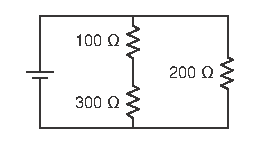
\includegraphics[keepaspectratio]{sample-AP1-Q02}
    \end{center}
    Which of the following correctly ranks the energy $E$ dissipated in the
        three resistors during a given time interval?
    \begin{choices}
        \wrongchoice{$E_{\SI{300}{\ohm}} > E_{\SI{200}{\ohm}} > E_{\SI{100}{\ohm}}$}
        \wrongchoice{$E_{\SI{300}{\ohm}} > E_{\SI{100}{\ohm}} > E_{\SI{200}{\ohm}}$}
      \correctchoice{$E_{\SI{200}{\ohm}} > E_{\SI{300}{\ohm}} > E_{\SI{100}{\ohm}}$}
        \wrongchoice{$E_{\SI{200}{\ohm}} > E_{\SI{100}{\ohm}} > E_{\SI{300}{\ohm}}$}
    \end{choices}
\end{question}
}


%% Sample AP 2 Questions
%%------------------------------
\element{AP}{
\begin{question}{sample2-Q01}
    The figure below shows four resistors in a circuit with a battery.
    \begin{center}
        \ctikzset{bipoles/length=0.75cm}
        \begin{circuitikz}
            \draw (0,0) to [battery] (0,2)
                        to [R,l=$3R$] (2,2)
                        to [R,l=$4R$] (4,2)
                        to [R,l=$R$]  (4,0)
                        to (0,0)
                  (4,2) to (6,2)
                        to [R,l=$2R$] (6,0)
                        to (4,0);
        \end{circuitikz}
        %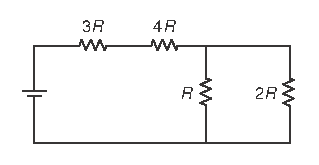
\includegraphics[keepaspectratio]{sample-AP2-Q01}
    \end{center}
    Which of the following correctly ranks the potential difference,
        $\delta V$, across the four resistors?
    \begin{choices}
        \wrongchoice{$\delta V_{4R} > \delta V_{3R} > \delta V_{2R} > \delta V_{R}$}
      \correctchoice{$\delta V_{4R} > \delta V_{3R} > \delta V_{2R} = \delta V_{R}$}
        \wrongchoice{$\delta V_{4R} = \delta V_{3R} > \delta V_{R} > \delta V_{2R}$}
        \wrongchoice{$\delta V_{2R} = \delta V_{R} > \delta V_{3R} > \delta V_{4R}$}
    \end{choices}
\end{question}
}


%% 2004-APB
%%------------------------------
\element{AP}{
\begin{question}{2004-APB-Q17}
    A wire of length $L$ and radius $r$ has a resistance $R$.
    What is the resistance of a second wire made from the same material
        that has a length $\frac{L}{2}$ and a radius $\frac{r}{2}$?
    \begin{multicols}{3}
    \begin{choices}
        \wrongchoice{$4 R$}
      \correctchoice{$2 R$}
        \wrongchoice{$R$}
        \wrongchoice{$\dfrac{R}{2}$}
        \wrongchoice{$\dfrac{R}{4}$}
    \end{choices}
    \end{multicols}
\end{question}
}

\element{AP}{
\begin{question}{2004-APB-Q18}
    The operating efficiency of a \SI{0.5}{\ampere}, \SI{120}{\volt}
        electric motor that lifts a \SI{9}{\kilo\gram} mass against
        gravity at an average velocity of \SI{0.5}{\meter\per\second}
        is most nearly.
    \begin{multicols}{3}
    \begin{choices}
        \wrongchoice{\SI{7}{\percent}}
        \wrongchoice{\SI{13}{\percent}}
        \wrongchoice{\SI{25}{\percent}}
        \wrongchoice{\SI{53}{\percent}}
      \correctchoice{\SI{75}{\percent}}
    \end{choices}
    \end{multicols}
\end{question}
}

\element{AP}{
\begin{question}{2004-APB-Q48}
    The diagram below has three resistors connected to a
        \SI{12}{\volt} battery.
    \begin{center}
        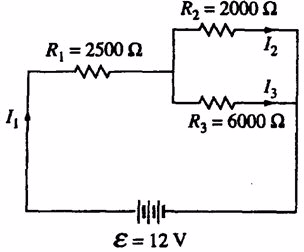
\includegraphics[keepaspectratio]{2004-APB-Q48}
    \end{center}
    What is the current $I_1$?
    \begin{multicols}{3}
    \begin{choices}
        \wrongchoice{\SI{800}{\milli\ampere}}
        \wrongchoice{\SI{600}{\milli\ampere}}
        \wrongchoice{\SI{400}{\milli\ampere}}
      \correctchoice{\SI{200}{\milli\ampere}}
        \wrongchoice{\SI{100}{\milli\ampere}}
    \end{choices}
    \end{multicols}
\end{question}
}

\element{AP}{
\begin{question}{2004-APB-Q49}
    The diagram below has three resistors connected to a
        \SI{12}{\volt} battery.
    \begin{center}
        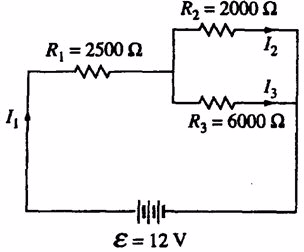
\includegraphics[keepaspectratio]{2004-APB-Q48}
    \end{center}
    How do the currents $I_1$, $I_2$, and $I_3$ compare?
    \begin{multicols}{2}
    \begin{choices}
      \correctchoice{$I_1 > I_2 > I_3$}
        \wrongchoice{$I_1 > I_3 > I_2$}
        \wrongchoice{$I_2 > I_1 > I_3$}
        \wrongchoice{$I_3 > I_1 > I_2$}
        \wrongchoice{$I_3 > I_2 > I_1$}
    \end{choices}
    \end{multicols}
\end{question}
}

